\section{Findings \& Discussion}

\epigraph{\justify``In God we trust, all others bring data.''}{Dr. William E. Demming(1900-1993)\\\textit{Columbia University}}

\subsection{Red-shift Regression}
\subsubsection{Phase I : Accuracy Assessment with Median Difference \label{rr1}}
The first phase initialised the learning on the regression problem where redshifts of galaxies were predicted using flux magnitudes across 5 colour indices. This was the foundational phase which constituted feature and target extraction from the dataset. The decision tree algorithm from the scikit-learn package's `DecisionTreeRegressor' to learn from the prepared dataset. The prediction was performed for input features from the same dataset. In order to assess the model's accuracy median of residuals i.e. the difference of actual and predicted value was used. Though the median residual strategy inherently did not have any problems with the precision of accuracy measurement, the problem was with the learning strategy. The 0 residual means that every prediction was successful. However, It was also unrealistic. This so because the training and testing set was a common one and the model was optimised to get the best results in the training set. The next phase of hold-out validation addressed these issues and a more realistic accuracy was obtained.

\subsubsection{Phase II: Realistic accuracy with hold-out validation} \label{rr2}
Extending from the foundational first phase, to get a more realistic assessment of the decision tree's performance hold-out validation was introduced in this phase. Contrary to the common training and testing set used in the first phase, the dataset in this phase was split into two - the training subset and the testing or the validation subset. The regressor learnt from the training set which contained the \inlinecode{Python}{train features} and the corresponding \inlinecode{Python}{target feature}. The prediction was done using the \inlinecode{python}{test features} of the training set. The median residual difference was calculated based on the difference of the model's target features produced during prediction and the actual target features.

The median difference of $\approx0.02$ was obtained. This means 50\% of the dataset have $< 0.02$ residual error in the prediction which is a significantly low number. This shows a high accuracy of the decision tree regressor. The reason for choosing the median of differences as the accuracy metric is that it gives a fair representation of the errors. Since the distribution residuals as seen below in figure \ref{fig: res}, is skewed, the median is a good approximate to take rather than another measure for example the mean.
\begin{figure}[H]
	\centering
	\includegraphics[width=\linewidth,keepaspectratio]{images/misc/residuals.png}
	\caption{Residual distribution with quartiles.}
	\label{fig:res}
\end{figure}

\subsubsection{Phase III: Improving the accuracy with K-Fold Cross Validation}\label{rr3}
The final phase  attempted to improve the accuracy of the classifier. The foremost approach to improving the accuracy of any machine learning model would be to increase the size of the training set. However, in this case, augmenting training size seems to have little impact on accuracy. As shown in the graph below in figure \ref{fig:dsg}, the median difference has difficulty surpassing the previously found accuracy of 0.02, even when the training size grows at 10 times the rate. Hence, for the training size of 25000, the accuracy limit has been reached.
\begin{figure}[H]
	\centering
	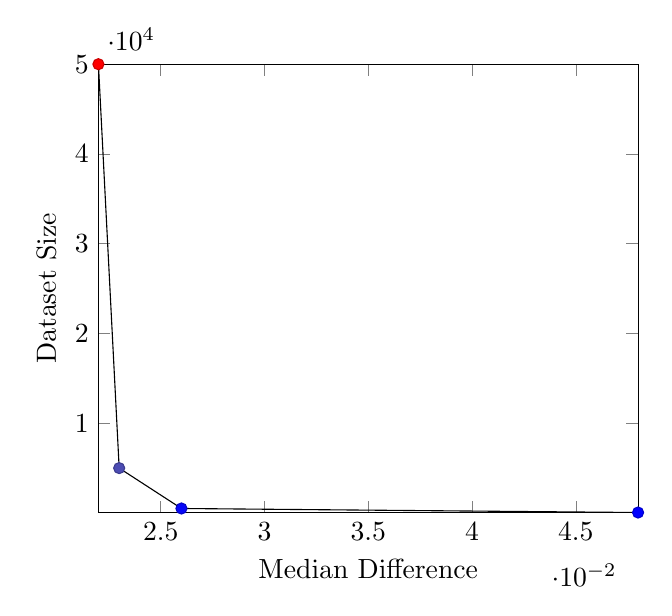
\begin{tikzpicture}
	\begin{axis}[enlargelimits=false, ylabel= Dataset Size, xlabel=Median Difference]
	\addplot+[scatter,mark=*,draw=black]
	table{
		0.048 50
		0.026 500
		0.023 5000
		0.022 50000
	};
	\end{axis}
	\end{tikzpicture}
	\caption{Rate of median difference change over the increasing dataset.}
	\label{fig:dsg}
\end{figure}
In order to further improve the accuracy, \textit{k}-fold cross-validation method was used. This not only improves the accuracy but also mitigates the overfitting problem of the decision tree, simultaneously. The following graph depicts the overfitting problem in the previous phase. As visualised below in figure \ref{fig:ofx}, as the tree depth increases, the model from the training set seem to have decreasing median residual or increasing performance. At a depth of 27, the errors seem to reduce to 0. On the other hand, the accuracy measure of the predictions on the test set though initially improves but eventually stars to overfit. In trying to account for the outliers it loses its general predictive accuracy.
\begin{figure}[H]
	\centering
	\includegraphics[width=\linewidth,keepaspectratio]{images/misc/ofit.png}
	\caption{Overfitting problem in decision tree visualised.}
	\label{fig:ofx}
\end{figure}
The chart below shown in \ref{fig:kch}visualises the accuracy of the decision tree regression classifier after the \textit{k}-fold cross validation. The dense points converge in a constant rate with occasional outliers.
\begin{figure}[H]
	\centering
	\includegraphics[width=\linewidth,keepaspectratio]{images/misc/k_fold_v.png}
	\caption{Visualisation of accuracy after \textit{k}-fold validation.}
	\label{fig:kch}
\end{figure}

\subsubsection{Quasars vs Galaxies}
The QSOs have greater median residual ($\approx0.074$) than the galaxies ($\approx0.016$). Possible reasons can be:
\begin{itemize}
	\item Fewer number of QSOs in the dataset(8525) than galaxies(41,475). 
	\item At SDSS flux may be feeble for SDSS at $\approx0.4$. This can create a measurement bias.
\end{itemize}
The median residual on a random sample of galaxies was \_diff of $\approx0.018$ which is slightly higher than the complete subset, but not sufficient to accommodate the gap between the two populations.

The figure below shows the normalised distribution function of the two populations.
\begin{figure}[H]
	\centering
	\includegraphics[width=\linewidth,keepaspectratio]{images/misc/redshift_distribution.png}
	\caption{Distribution of redshifts of galaxies and quasars}
	\label{fig:qrg}
\end{figure}
The majority of galaxies accumulate at 0.10 to form a peak while the quasars are spread out and evenly distributed out up to redshift $\approx 2.5$. This could result in measurement bias. In the case of the galaxies, the decision tree is trained to approximate around 0.4. As such the predictions from this model will not be larger than the maximum target value. So the maximum difference (or residual) for each galaxy in this set will be a lot smaller than the maximum residual for the QSOs.

A clearer view of this by looking at the predicted redshifts vs actual redshifts in the following plot.
\begin{figure}[H]
	\centering
	\includegraphics[width=\linewidth,keepaspectratio]{images/misc/predicted_actual_qso.png}
	\caption{Predicted vs measured redshifts of galaxies and quasars.}
	\label{fig:prq}
\end{figure}

\subsection{Morphology Classification}

\subsubsection{Accuracy Assessment with Confusion Matrix} \label{mc1}
\begin{figure}[H]
	\centering
	\includegraphics[width=\linewidth,keepaspectratio]{images/misc/confusion_matrix.png}
	\caption{Confusion matrix for elliptical, mergers, spiral galaxies.}
	\label{fig:cfm}
\end{figure}

The x-axis represents the predicted classes and the y-axis represents the correct classes. The value in each cell is the number of examples with those predicted and actual classes. Correctly classified objects are along the diagonal of the matrix. So of the 260 actual spirals (correct class) in the data set, 200 are correctly predicted as spirals, 3 are incorrectly predicted as ellipticals and 57 are incorrectly predicted as mergers.The sum along each row or column can be used to get the totals of true and predicted classes. So for example, by summing each of the rows it can be confirmed there are 260 mergers, 260 spirals and 260 ellipticals in the data set.

\subsubsection{Random Forest vs Decision Tree}
Did the random forest improve the accuracy of the model? The answer is yes – we see a substantial increase in accuracy. When we look at the 10-fold cross validation results, we see that the random forest systematically out-performs a single decision tree:
\begin{table}[h]
	\centering
	\begin{adjustbox}{width=\linewidth}
	\begin{tabular}{rll}
		\textbf{Metric} & \textbf{Random Forest} & \textbf{Decision Tree}\\
		\hline
		Median score (\textit{\small{Mdn}}) & 0.865 & 0.775\\
		Mean score ($\mu$) & 0.867 & 0.792\\
		Standard deviation of scores ($\sigma$) & 0.036 & 0.035
	\end{tabular}
	\end{adjustbox}
	\caption{Performance of Random Forest vs Decision Tree}
\end{table}

\begin{figure}[H]
	\centering
	\begin{subfigure}{.5\linewidth}
		\centering
		\includegraphics[width=\linewidth, keepaspectratio]{images/misc/confusion_matrix.png}
		\caption{Confusion Matrix of Decision Tree.}
		\label{fig:sub1}
	\end{subfigure}%
	\begin{subfigure}{.5\linewidth}
		\centering
		\includegraphics[width=\linewidth, keepaspectratio]{images/misc/rf_cm.png}
		\caption{Confusion Matrix of Random Forest}
		\label{fig:sub2}
	\end{subfigure}
	\caption{A comparison between prediction accuracy for decision tree and ensemble method used in morphologic classification of galaxies.}
	\label{fig:test}
\end{figure}

The random forest is around ~6-7\% more accurate than a standard decision tree. The figure above depicts a side-by-side comparison of the confusion matrices from the galaxy catalogues. The second showing the results for the random forest classifier and the first for the decision tree classifier. There are improvements across the board with the biggest improvement (percentage) observed between ellipticals and spirals.